\documentclass[14pt]{beamer}
\usetheme{Madrid} % My favorite!
%\usetheme{Boadilla} % Pretty neat, soft color.
%\usetheme{default}
%\usetheme{Warsaw}
%\usetheme{Bergen} % This template has nagivation on the left
%\usetheme{Frankfurt} % Similar to the default 
%with an extra region at the top.
%\usecolortheme{seahorse} % Simple and clean template
%\usetheme{Darmstadt} % not so good
% Uncomment the following line if you want %
% page numbers and using Warsaw theme%
% \setbeamertemplate{footline}[page number]
%\setbeamercovered{transparent}
\setbeamercovered{invisible}
% To remove the navigation symbols from 
% the bottom of slides%
\setbeamertemplate{navigation symbols}{} 
%
\usepackage{graphicx}
\usepackage{mathtools}
\usepackage{cancel}
\usepackage{algorithm2e}

\usepackage{pifont}% http://tex.stackexchange.com/questions/42619/x-mark-to-match-checkmark
\newcommand{\cmark}{\ding{51}}%
\newcommand{\xmark}{\ding{55}}%
\newcommand{\inprogress}{\ding{224}}%

\usepackage{xcolor}

\definecolor{olive}{rgb}{0.3, 0.4, .1}
\definecolor{fore}{RGB}{249,242,215}
\definecolor{back}{RGB}{51,51,51}
\definecolor{title}{RGB}{255,0,90}
\definecolor{dgreen}{rgb}{0.,0.6,0.}
\definecolor{gold}{rgb}{1.,0.84,0.}
\definecolor{JungleGreen}{cmyk}{0.99,0,0.52,0}
\definecolor{BlueGreen}{cmyk}{0.85,0,0.33,0}
\definecolor{RawSienna}{cmyk}{0,0.72,1,0.45}
\definecolor{Magenta}{cmyk}{0,1,0,0}

\linespread{1.5}

%\usepackage{bm}         % For typesetting bold math (not \mathbold)
%\logo{\includegraphics[height=0.6cm]{yourlogo.eps}}
%
\title[ToasterBooster]{Using LMS Inside New Backend for DBToaster (DDBToaster)}
\author{Thierry Coppey, Mohammad Dashti}
\institute[EPFL]
{
Ecole Polytechnique Federale de Lausanne\\
\medskip
{\emph{[first.last]@epfl.ch}}
}
\date{\today}
% \today will show current date. 
% Alternatively, you can specify a date.
%
\begin{document}
%
\begin{frame}
\titlepage
\end{frame}
%

%
\begin{frame}
\frametitle{First: DBToaster Alone}
\includegraphics[width=\textwidth]{DBToasterHighLevel}
\end{frame}
%

%
\begin{frame}
\frametitle{Then: ToasterBooster}
\fontsize{18pt}{12}\selectfont
\begin{itemize}
\item It is a separate optimization module
\end{itemize}
\includegraphics[width=\textwidth]{DBToasterHighLevelUsingToasterBooster}
\end{frame}
%

%
\begin{frame}
\frametitle{Now: DDBToaster}
\fontsize{18pt}{12}\selectfont
\begin{itemize}
\item A new back-end for DBToaster
\item Compiles M3 programs into Scala
\item Uses CPS style
\end{itemize}
\includegraphics[width=\textwidth]{DBToasterHighLevelUsingDDBToaster}
\end{frame}
%

%
\begin{frame}
\frametitle{Achievements}
%\fontsize{18pt}{12}\selectfont
\begin{itemize}
\item New back-end passes all available test cases (thanks to Thierry's hard work)
\item New back-end is faster than the previous one, in almost all cases
\item Eliminating one costly compilation phase (between DBToaster and ToasterBooster)

\end{itemize}
\end{frame}

%
\begin{frame}
\frametitle{Experimental Results}

\includegraphics[width=\textwidth]{finance-standard-concise}

\end{frame}

%
\begin{frame}
\frametitle{EoF}
\begin{center}
Questions?
\end{center}

\end{frame}


%
\begin{frame}[noframenumbering]
\frametitle{What is CPS?}
%\fontsize{18pt}{12}\selectfont
\begin{itemize}
\item Continuation = "the rest of the program"
\item Example:
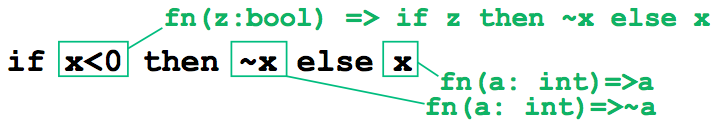
\includegraphics[width=0.9\textwidth]{CPS1}
\pause
\item So we can rewrite the above code as:
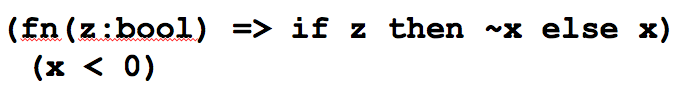
\includegraphics[width=0.9\textwidth]{CPS2}

\end{itemize}
\end{frame}

% End of slides

%\section{References}
%\begin{frame}%[allowframebreaks]
%  \frametitle{References}
%  \begin{tiny}
%	\begin{thebibliography}{99}

%books
\beamertemplatebookbibitems
\bibitem{AMA2006} [AMA06] José Nelson Amaral, "TopicC: Loop Fusion" slides, Compiler Design and Optimization, Department of Computing Science, University of Alberta, 2006. URL: http://webdocs.cs.ualberta.ca/~amaral/courses/680/.


\beamertemplatearticlebibitems

\bibitem{MEG1997} [MEG97] Nimrod Megiddo and Vivek Sarkar. 1997. Optimal weighted loop fusion for parallel programs. In Proceedings of the ninth annual ACM symposium on Parallel algorithms and architectures (SPAA '97). ACM, New York, NY, USA, 282-291.

\bibitem{GAO92} [GAO92] G. R. Gao, R. Olsen, V. Sarkar, and R. Thekkath. 1993. Collective loop fusion for array contraction. Springer-Verlag Lecture Notes in Computer Science, 757. Proceedings of the Fifth Workshop on Languages and Compilers for Parallel Computing, Yale University, 281-295.
\bibitem{KEN93} [KEN93] Ken Kennedy and Kathryn S. McKinley. 1994. Maximizing Loop Parallelism and Improving Data Locality via Loop Fusion and Distribution. Springer-Verlag Lecture Notes in Computer Science, 768. Proceedings of the Sixth Workshop on Languages and Compilers for Parallel Computing, Portland, Oregon, 301-320.

\end{thebibliography}

%  \end{tiny}
%\end{frame}

\end{document} 